\chapter{Services}

I \textit{Services} sono componenti di un'applicazione che eseguono operazioni in \textit{background} senza fornire una interfaccia grafica. \\
Una qualsiasi componente può lanciarne uno ed esso rimarrà attivo in \textit{background} anche se l'untente passa ad un altra app.\\
Inoltre, tramite l'operazione di \textit{bind}, una componente può essere associata ad un servizio per poterci comunicare o effettuare operazioni di IPC (Inter Process Comunication).\\
È buona norma usare un \textit{service} per:
\begin{itemize}
	\item Completare operazioni lanciate dall'utente: terminare un \textit{download}/\textit{upload}, riprodurre musica etc.
	\item Effettuare operazioni senza interventi sulla UI. Ad esempio è possibile controllare periodicamente l'accelerometro del dispositivo per monitorare se l'utente è fermo, sta camminando o sta correndo.
	\item "Comunicare" al sistema operativo che l'applicazione ha del lavoro da fare in background e quindi evitare che l'OS deallochi i processi prima che abbiano terminato.
\end{itemize}

\section{Lifecycle}
\begin{figure}
    \centering
    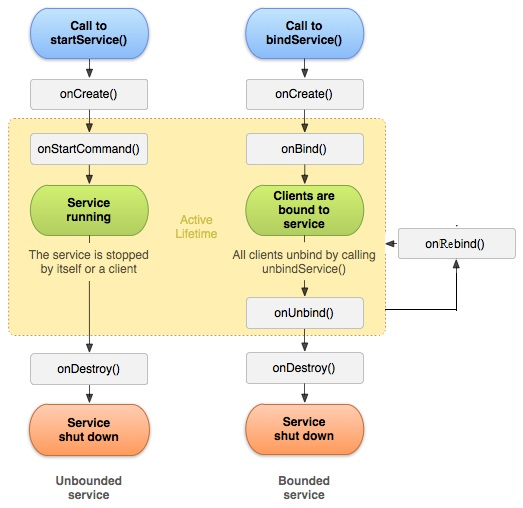
\includegraphics[scale=0.6]{service_lifecycle}
    \caption{Service Lifecycle}
    \label{fig:my_label}
\end{figure}
Per creare un servizio è necessario estendere la classe \texttt{Service}. Nell'implementazione bisogna effettuare l'\textit{override} dei suoi \textit{callback} per gestire il suo ciclo di vita. Una lista dei principali:
\begin{itemize}
	\item \texttt{onStartCommand()}\\
	Questo metodo è chiamato quando un'altra componente (ad esempio una \textit{Activity}) richiede esplicitamente di lanciare il servizio tramite \texttt{startService()}. Quando viene eseguito questo metodo il servizio parte e può continuare indefinitamente: per fermarlo è necessario chiamare \texttt{stopSelf()} o \texttt{stopService()}. Se vuoi solo fornire \textit{binding} non serve overridare questo metodo.
	\item \texttt{onBind()}\\
	Questo metodo è chiamato quando un'altra componente chiede di associarsi con il servizio tramite il metodo \texttt{bindService()}. L'implementazione di questo metodo deve fornire una interfaccia di comunicazione ritornando un \texttt{IBinder}; che di solito rappresenta una interfaccia di comunicazione complessa che è stata descritta tramite AIDL. Questo metodo deve essere necessariamente implementato; se non vuoi dare la possibilità di effettuare binding, ritorna \texttt{null}.
	\item \texttt{onCreate()}\\
	Il sistema chiama questo metodo per effettuare il setup iniziale (che viene eseguito una sola volta per servizio). Viene eseguito prima sia di \texttt{onStartCommand()} che di \texttt{onBind()}. Se il servizio è già \textit{running} questo metodo non viene chiamato.
	\item \texttt{onDestroy()}\\
	In sistema invoca questo metodo quando il servizio non non è più usato e viene distrutto. Nell'implementazione è necessario deallocare tutte le risorse come \textit{thread}, \textit{listener} e \textit{receiver}. È l'ultima chiamata che riceve il servizio.
\end{itemize}

\section{Dichiarare un Service nel manifest}
Ogni servizio deve essere dichiarato nel \textit{manifest} aggiungendo un elemento \texttt{<service>} come figlio di \texttt{<application>}.
\begin{lstlisting}[language=XML]
<manifest ... >
  ...
  <application ... >
      <service android:name=".ExampleService" />
      ...
  </application>
</manifest>
\end{lstlisting}

L'elemento \texttt{<service>} può include altri attributi usati, ad esempio, per definire proprietà come i permessi necessari per lanciare il servizio o i processi in cui il servizio deve essere \textit{runnato}.\\
L'unico attributo obbligatorio è \texttt{android:name}: specifica ovviamente il nome del servizio e deve rimanere sempre invariato per evitare il rischio di bug nel caso di dipendenze, start espliciti o \textit{binding}.\\
Ad esempio un servizio può essere dichiarato come segue:
\begin{lstlisting}[language=XML]
<service android:description="string resource"
         android:directBootAware=["true" | "false"]
         android:enabled=["true" | "false"]
         android:exported=["true" | "false"]
         android:icon="drawable resource"
         android:isolatedProcess=["true" | "false"]
         android:label="string resource"
         android:name="string"
         android:permission="string"
         android:process="string" >
    . . .
</service>
\end{lstlisting}



\section{Tipi di Servizi}
I serivizi si possono dividere in tre tipologie:
\begin{itemize}
	\item \textbf{Scheduled}: Questi \textit{services} sono fatti partire da una API come il \texttt{JobScheduler}. Uno scheduler lancia i servizi a lui associati al verificarsi di alcune condizioni temporali e di \textit{network}.\\
	N.B. \texttt{JobScheduler} è disponibile solo da Android 5.0 (API 21) in poi.
	\item \textbf{Started}: Un servizio è \textit{started} quando viene fatto partire esplicitamente da un'altra componente tramite una chiamata a \texttt{startService()}. Quando un servizio è lanciato in questo modo esegue indefinitamente, anche nel caso in cui il componente che l'ha lanciato venga distrutto. Generalmente esegue una singola operazione (come completare un \textit{download}) e poi è sua responsabilità autosospendersi. 
	\item \textbf{Bound}: Un servizio è \textit{bound} quando un'altra componente gli viene associata tramite una chiamata a \texttt{bindService()}. Offre una interfaccia \textit{client-server} che permette alle componenti di interagire con il servzio, mandare richieste, ricevere risultati o addirittura effettuare IPC. Un servizio di questo tipo continua solamente fino a quando ha componenti associate, quando tutte le componenti si sono disassociate esso termina.
\end{itemize}


La caratterizzazione non è rigida: ad esempio un servizio può essere \textit{started}, ma anche permettere il \textit{binding}. Basta implementare sia \texttt{onStartCommand()} che \texttt{onBind()} quando si sta ridefinendo il \textit{lifecycle}.\\
Tutti i servizi risiedono nel \textit{main thread}, quindi non se si deve fare \textit{networking} o operazioni \textit{CPU-intensive} sarà necessario creare un nuovo \textit{thread} all'interno del \textit{service}.


\subsection{Started Services}
Sono servizi lanciati da un'altra componente tramite \texttt{startService()}, che risulta in una chiamata a \texttt{onStartCommand()}. La componente che lo lancia deve passargli un \texttt{Intent} che specifica il servizio e contiene tutti i dati necessari per la sua esecuzione.\\
Una volta partito ha un ciclo di vita indipendente dalla componente genitrice, quindi può \textit{runnare} indefinitamente in \textit{background} ed è sua responsabilità chiamare \texttt{stopSelf()} oppure deve essere un'altra componente a chiamare \texttt{stopService()}.\\
Le due principali classi che possono essere estese per creare uno \textit{started service} sono:
\begin{itemize}
	\item \texttt{Service}: è la classe base da cui estendono tutti i \textit{service}. Di dafult vive sul \textit{main thread}, quindi se deve effettuare operazione computazionalmente pesanti oppure \textit{networking} è necessario creare un altro \textit{thread}.
	\item \texttt{IntentService}: è una sottoclasse di \texttt{Service} che usa uno \textit{worker thread} per eseguire tutte le richieste. Estendere questa classe è la scelta migliore nel caso non si debbano gestire più richieste simultaneamente.
\end{itemize}

\subsubsection{Estendere IntentService}
La più comune implementazione di un servizio è tramite la superclasse \texttt{IntentService}.
Questa classe esegue le seguenti operazioni:
\begin{itemize}
	\item Crea un \textit{default worker} che esegue tutti gli \textit{intent} specificati in \texttt{onStartCommand()} separatamente dall'\textit{UI-thread}.
	\item Crea una coda di \textit{intent} da passare uno alla volta alla implentazione del metodo \texttt{onHandleIntent()} (di questa classe). In questo modo non ci saranno problemi di \textit{multithreading}.
	\item Ferma il servizio dopo che tutte le richieste sono state processate, così non c'è bisogno di chiamare esplicitamente \texttt{stopSelf()}.
	\item Fornisce una implementazione di default di \texttt{onBind()} che ritorna \texttt{null}, ovvero non permette il \textit{binding}.
	\item Fornisce una implementazione di default di \texttt{onStartCommand()} che semplicemente inoltra le richieste alla propria implementazione di \texttt{onHandleIntent()}.
\end{itemize}

Per estendere la classe è necessario solamente un construttore e l'\textit{overrinding} di \texttt{onHandleIntent()}, come nell'esempio:

\begin{lstlisting}[language=Java]
public class HelloIntentService extends IntentService {

  /**
   * A constructor is required, and must call the super IntentService(String)
   * constructor with a name for the worker thread.
   */
  public HelloIntentService() {
      super("HelloIntentService");
  }

  /**
   * The IntentService calls this method from the default worker thread with
   * the intent that started the service. When this method returns, IntentService
   * stops the service, as appropriate.
   */
  @Override
  protected void onHandleIntent(Intent intent) {
      // Normally we would do some work here, like download a file.
      // For our sample, we just sleep for 5 seconds.
      try {
          Thread.sleep(5000);
      } catch (InterruptedException e) {
          // Restore interrupt status.
          Thread.currentThread().interrupt();
      }
  }
}
\end{lstlisting}

Se c'è la necessità di fare l'\textit{override} di altri metodi come \texttt{onCreate()}, \texttt{onStartCommand()} o \texttt{onDestroy()} è necessario chiamare l'implementazione della superclasse per fare un modo che \texttt{IntentService} gestica oppurtunamente il ciclo di vita dello \textit{worker thread}.\\
Ad esempio questo potrebbe essere un \textit{override} di \texttt{onStartCommand()}.
\begin{lstlisting}[language=Java]
@Override
public int onStartCommand(Intent intent, int flags, int startId) {
    Toast.makeText(this, "service starting", Toast.LENGTH_SHORT).show();
    return super.onStartCommand(intent,flags,startId);
}
\end{lstlisting}

Se si vuole permettere il \textit{binding} è necessario fare l'\textit{override} di \texttt{onBind()} e non chiamare l'implementazione della superclasse perché altrimenti ritornerebbe \texttt{null}.\\


\subsubsection{Estendere Serice}
Se il servizio deve gestire più richieste simultaneamente si rende necessario estendere la classe \texttt{Service}.\\
Per confronto questo è un esempio di un servizio con lo stesso comportamento di quello dell'esempio precedente ma implementato usando \texttt{Service}.

\begin{lstlisting}[language=Java]
public class HelloService extends Service {
  private Looper mServiceLooper;
  private ServiceHandler mServiceHandler;

  // Handler that receives messages from the thread
  private final class ServiceHandler extends Handler {
      public ServiceHandler(Looper looper) {
          super(looper);
      }
      @Override
      public void handleMessage(Message msg) {
          // Normally we would do some work here, like download a file.
          // For our sample, we just sleep for 5 seconds.
          try {
              Thread.sleep(5000);
          } catch (InterruptedException e) {
              // Restore interrupt status.
              Thread.currentThread().interrupt();
          }
          // Stop the service using the startId, so that we don't stop
          // the service in the middle of handling another job
          stopSelf(msg.arg1);
      }
  }

  @Override
  public void onCreate() {
    // Start up the thread running the service.  Note that we create a
    // separate thread because the service normally runs in the process's
    // main thread, which we don't want to block.  We also make it
    // background priority so CPU-intensive work will not disrupt our UI.
    HandlerThread thread = new HandlerThread("ServiceStartArguments",
            Process.THREAD_PRIORITY_BACKGROUND);
    thread.start();

    // Get the HandlerThread's Looper and use it for our Handler
    mServiceLooper = thread.getLooper();
    mServiceHandler = new ServiceHandler(mServiceLooper);
  }

  @Override
  public int onStartCommand(Intent intent, int flags, int startId) {
      Toast.makeText(this, "service starting", Toast.LENGTH_SHORT).show();

      // For each start request, send a message to start a job and deliver the
      // start ID so we know which request we're stopping when we finish the job
      Message msg = mServiceHandler.obtainMessage();
      msg.arg1 = startId;
      mServiceHandler.sendMessage(msg);

      // If we get killed, after returning from here, restart
      return START_STICKY;
  }

  @Override
  public IBinder onBind(Intent intent) {
      // We don't provide binding, so return null
      return null;
  }

  @Override
  public void onDestroy() {
    Toast.makeText(this, "service done", Toast.LENGTH_SHORT).show();
  }
}
\end{lstlisting}

Il metodo \texttt{onStartCommand()} deve ritornare un intero che rappresenta il modo in cui il servizio deve continuare nel caso che il sistema lo uccida. I possibili modi sono:

\begin{itemize}
	\item \texttt{START\_NOT\_STICKY}: Il sistema non ricrea il servizio a meno che non ci siano rischieste pendenti. È la soluzione più \textit{safe} per evitare che il servizio continui indefinitamente.
	\item \texttt{START\_STICKY}: Il sistema ricrea il servizio, ma non gli riconsegna l'ultimo \textit{intent}. Il sistema gli da in pasto tutti i \textit{pending intent} o eventualmente \texttt{null} se la coda era vuota.
	Questa cosa è adatta per servizi come i \textit{media player} che non eseguono comandi ma girano indefinitamente in attesa di un \textit{job}.
	\item \texttt{START\_REDELIVER\_INTENT}: Come il precedente ma il sistema gli riconsegna anche l'ultimo \textit{intent}. Questa modalità è adatta a servizi che eseguono attivamente \textit{job} che devono essere rapidamente ricominciati (come i \textit{download}).
\end{itemize}

\subsection{Bound Services}
Permettono alle altre componenti del sistema di associarsi chiamando \texttt{bindSerice()}, generalmente non permettono di far partire il servizio chiamando \texttt{startSerice()}. Permettono, invece, di avere interazioni da parte di altre componenti attraverso IPC (\textit{Inter Process Communication}).\\
Per creare un \textit{bound service} è necessario fare l'\textit{override} di \texttt{onBind()}, che deve ritornare un \texttt{IBinder} che specifichi l'interfaccia di comunicazione.\\
Le altre componenti si possono associare chiamando \texttt{bindService()} e disassociare chiamando \texttt{unbindService()}.\\
Quando un \textit{bound service} non ha più componenti associate viene distrutto, non è necessario fermarlo esplicitamente.


\subsection{Starting a Service}
Per far partire un \textit{service} da un'\texttt{Activity} si può fare come nell'esempio:
\begin{lstlisting}[language=Java]
Intent intent = new Intent(this, HelloService.class);
startService(intent)
\end{lstlisting}

Il metodo \texttt{startService()} ritorna immediatamente. Se il servizio non fornisce \textit{binding} l'\textit{intent} fornito a \texttt{startService()} è l'unica via di comunicazione con il servizio. Se si vogliono comunque avere dei risultati è consigliabile usare un \texttt{PendingIntent}.





\chapter{Broadcast Receivers}

Un servizio \textit{running} può notificare l'utente in due modi: una \textit{toast notification} oppure una \textit{status bar notification}.

\section{Toast Notifications}
Sono notifiche che appaiono per un breve periodo prima di scomparire. Possono avere durata lunga o corta e una gravità per decidere in quale porzione dello schermo debbano essere visualizzate.

\begin{lstlisting}[language=Java]
Toast toast = Toast.makeText(
		getApplicationContext(),
		"I am a Toast!",
		Toast.LENGTH_SHORT);
toast.setGravity(Gravity.TOP|Gravity.LEFT, 0, 0);
toast.show();
\end{lstlisting}


\section{Status Bar Notifications}
Sono mostrate al di fuori della normale UI, sulla barra delle notifiche.\\
Un oggetto notifica deve contenere una piccola icona (\texttt{setSmallIcon()}), un titolo (\texttt{setContentTitle()}), un testo dettagliato (\texttt{setContentText()}) ed opzionalmente una azione.\\
Una azione fornisce un utente per andare direttamente dalla zona delle notifiche ad una \textit{Activity} dell'applicazione.\\
Per costruire una notifica è necessario usare un \textit{builder} come segue:
\begin{lstlisting}[language=Java]
Intent notificationIntent = new Intent(this, ExampleActivity.class);
PendingIntent pendingIntent = PendingIntent.getActivity(this, 0, notificationIntent, 0);

Notification notification = new Notification.Builder(this)
    .setContentTitle(getText(R.string.notification_title))
    .setContentText(getText(R.string.notification_message))
    .setSmallIcon(R.drawable.icon)
    .setContentIntent(pendingIntent)
    .setTicker(getText(R.string.ticker_text))
    .build();

\end{lstlisting}

Per far partire la notifica invece usare il \texttt{NotificationManager}:
\begin{lstlisting}[language=Java]
NotificationManager mNotificationManager =
    (NotificationManager) getSystemService(Context.NOTIFICATION_SERVICE);
// mId allows you to update the notification later on.
mNotificationManager.notify(mId, mBuilder.build());

\end{lstlisting}

\section{Ricevere Notifiche}
Le applicazioni \textit{Android} possono mandare o ricevere messaggi sal sistema in maniera simile al pattern \textit{publish-subscribe}.\\
I messaggi sono inviati quando succedono "eventi importanti": ad esempio quando il sistema si è avviato, oppure è iniziata la carica; inoltre le applicazioni possono notificare eventi personalizzati.\\
Le applicazioni possono registrarsi per ricevere i \textit{broadcast} a cui sono interessate; il sistema si occupa automaticamente di reindirizzare i corretti messaggi ai corretti destinatari.\\
Le applicazioni possono ricevere \textit{broadcast} in due modi:

\subsection{Manifest-declared Receivers}
Si possono dichiarare dei \textit{receivers} nel \textit{manifest}, in questo modo l'app si registra all'istallazione.
\begin{lstlisting}[language=XML]
<receiver android:name=".MyBroadcastReceiver"  android:exported="true">
    <intent-filter>
        <action android:name="android.intent.action.BOOT_COMPLETED"/>
        <action android:name="android.intent.action.INPUT_METHOD_CHANGED" />
    </intent-filter>
</receiver> 
\end{lstlisting}


\subsection{Context-registered receiver}
Ricevono i \textit{broadcast} fino a quando il loro contesto è valido. Ad esempio se si registra il \textit{receiver} al contesto di una \textit{activity} rimarrà attivo fino alla distruzione dell'\textit{activity}.\\

\begin{lstlisting}[language=Java]
public class MyBroadcastReceiver extends BroadcastReceiver {
    private static final String TAG = "MyBroadcastReceiver";
    @Override
    public void onReceive(Context context, Intent intent) {
        StringBuilder sb = new StringBuilder();
        sb.append("Action: " + intent.getAction() + "\n");
        sb.append("URI: " + intent.toUri(Intent.URI_INTENT_SCHEME).toString() + "\n");
        String log = sb.toString();
        Log.d(TAG, log);
        Toast.makeText(context, log, Toast.LENGTH_LONG).show();
    }
}

BroadcastReceiver br = new MyBroadcastReceiver();

IntentFilter filter = new IntentFilter(ConnectivityManager.CONNECTIVITY_ACTION);
intentFilter.addAction(Intent.ACTION_AIRPLANE_MODE_CHANGED);
this.registerReceiver(br, filter);
\end{lstlisting}

Per smettere di ricevere le notifiche da un \textit{broadcast} basta chiamare \texttt{unregisterReceiver()}.\\
Nota bene:
\begin{itemize}
	\item Nel caso ci si registri dentro \texttt{onCreate()} bisogna disiscriversi in \texttt{onDestroy()} per evitare \textit{memory leaks}.
	\item Nel caso ci si registri dentro \texttt{onResume()} bisogna disiscriversi in \texttt{onPause()} per evitare di registrarsi più volte.
\end{itemize}


\subsection{Ricevere messaggi Asincronamente}
Di default il metodo \texttt{onReceive()} vive sull'\textit{UI-thread}. Per renderlo asincrono si può fare come segue:

\begin{lstlisting}[language=Java]
public class MyBroadcastReceiver extends BroadcastReceiver {
    private static final String TAG = "MyBroadcastReceiver";

    @Override
    public void onReceive(final Context context, final Intent intent) {
        final PendingResult pendingResult = goAsync();
        AsyncTask<String, Integer, String> asyncTask = new AsyncTask<String, Integer, String>() {
            @Override
            protected String doInBackground(String... params) {
                StringBuilder sb = new StringBuilder();
                sb.append("Action: " + intent.getAction() + "\n");
                sb.append("URI: " + intent.toUri(Intent.URI_INTENT_SCHEME).toString() + "\n");
                Log.d(TAG, log);
                // Must call finish() so the BroadcastReceiver can be recycled.
                pendingResult.finish();
                return data;
            }
        };
        asyncTask.execute();
    }
}
\end{lstlisting}


\section{Inviare Broadcast}
\textit{Android} fornisce tre metodi per inviare \textit{broadcast}:

\begin{itemize}
	\item \texttt{sendOrderedBroadcast(Intent, String)}\\
	Il metodo manda i \textit{broadcast} ad un \textit{receiver} alla volta. Dato che i \textit{receiver} ricevono il messaggio a turno ognuno può decidere se propagarlo, oppure abortire completamente il passaggio del \textit{broadcast}. L'ordine di priorità dei riceventi può essere modificato dal \textit{manifest} usando l'attributo \texttt{android:priority}.
	\item \texttt{sendBroadcast(Intent)}\\
	Manda il \textit{broadcast} a tutti i \textit{receiver} in ordine non prefissato. Ciò significa che i riceventi non possono propagare i risultati ed abortire il processo; ma è più efficiente.
	\item \texttt{LocalBroadcastManager.sendBroadcast}\\
	Manda il messaggio ai soli \textit{receiver} all'interno della stessa applicazione. Molto efficiente e permette di non considerare le implicazioni di sicurezza dovute ad app esterne.
\end{itemize}

\subsection{Filtrare tramite permessi}
\subsubsection{In invio}
\textit{Android} permette di restringere i \textit{broadcast} tramite permessi. quando si invia un \textit{broadcast} si può specificare un set di permessi che il ricevente deve avere per poter ricevere il messaggio.\\
Ad esempio se il \textit{broadcast} è inviato in questa maniera:
\begin{lstlisting}[language=Java]
sendBroadcast(new Intent("com.example.NOTIFY"),
              Manifest.permission.SEND_SMS);
\end{lstlisting}
Potrà essere ricevuto solo da \textit{receiver} che abbiano nel \textit{manifest}:
\begin{lstlisting}[language=XML]
<uses-permission android:name="android.permission.SEND_SMS"/>
\end{lstlisting}

\subsubsection{In ricezione}
Anche in ricezione si possono porre restrizioni.\\
Ad esempio se l'app destinataria dichiara nel \textit{manifest} queste linee:
\begin{lstlisting}[language=XML]
<receiver android:name=".MyBroadcastReceiver"
          android:permission="android.permission.SEND_SMS">
    <intent-filter>
        <action android:name="android.intent.action.AIRPLANE_MODE"/>
    </intent-filter>
</receiver>
\end{lstlisting}
E possiede un \textit{context-registered receiver} del tipo:
\begin{lstlisting}[language=Java]
IntentFilter filter = new IntentFilter(Intent.ACTION_AIRPLANE_MODE_CHANGED);
registerReceiver(receiver, filter, Manifest.permission.SEND_SMS, null );
\end{lstlisting}
Allora l'applicazione mittente per poter comunicare con quest'ultima dovrà richiedere i permessi per inviare gli SMS:
\begin{lstlisting}[language=XML]
<uses-permission android:name="android.permission.SEND_SMS"/>
\end{lstlisting}